\documentclass[11pt]{article}

\usepackage{latexsym}
\usepackage{amsmath}
\usepackage{amssymb}
\usepackage{amsthm}
\usepackage{graphicx}
\usepackage{wrapfig}
\usepackage{pseudocode}
\usepackage{url}
\usepackage[backref, colorlinks=true, citecolor=red, urlcolor=blue, pdfauthor={Jyh-Ming Lien}]{hyperref}


\newcommand{\handout}[5]{
  \noindent
  \begin{center}
  \framebox{
    \vbox{
      \hbox to 5.78in { {\bf } \hfill #2 }
      \vspace{4mm}
      \hbox to 5.78in { {\Large \hfill #5  \hfill} }
      \vspace{2mm}
      \hbox to 5.78in { {\em #3 \hfill #4} }
    }
  }
  \end{center}
  \vspace*{4mm}
}

\newcommand{\lecture}[4]{\handout{#1}{#2}{#3}{}{Report for #1}}

\newtheorem{theorem}{Theorem}
\newtheorem{corollary}[theorem]{Corollary}
\newtheorem{lemma}[theorem]{Lemma}
\newtheorem{observation}[theorem]{Observation}
\newtheorem{proposition}[theorem]{Proposition}
\newtheorem{definition}[theorem]{Definition}
\newtheorem{claim}[theorem]{Claim}
\newtheorem{fact}[theorem]{Fact}
\newtheorem{assumption}[theorem]{Assumption}

% 1-inch margins, from fullpage.sty by H.Partl, Version 2, Dec. 15, 1988.
\topmargin 0pt
\advance \topmargin by -\headheight
\advance \topmargin by -\headsep
\textheight 8.9in
\oddsidemargin 0pt
\evensidemargin \oddsidemargin
\marginparwidth 0.5in
\textwidth 6.5in

\parindent 0in
\parskip 1.5ex
%\renewcommand{\baselinestretch}{1.25}

\begin{document}

\lecture{Advance Algorithm Programming Assignment 1 Part2: 3D $\alpha$-shape }{Fall 2015}{Moran Kim}


\section{Implementation Details}
To implement Delaunay triangulation in 3-dimension, I used 'QHull()' to compute covex hull of the vertices in 4-dimension.
Given set of vertices $V=\{(v_x,v_y,v_z)\in\mathbb{R}^3|\hspace{0.15cm} for\hspace{0.15cm} v_x,v_y,v_z\in\mathbb{R}\}$, we lift up the points v$\in V$ by adding additional component $V_m=(v_x)^2+(v_y)^2+(v_z)^2$. Let us denote $V4={(v_x,v_y,v_z,v_m)\in\mathbb{R}^4}$. Then we can construct a convex hull of V4 which is a composition of tetrahedrons. After computing the convex hull of V4, we select the vertices of the tetrahedron whose facing direction is downside. After storing the information of that selected vertices $v_{selected}\in V4$, we draw tetrahedron of $v_{selected}$ with the part of Qhull() which is Delaunay(). I assumed that the facet of the Deluanay triangulation is the face of convex hull of points that are lifted up in 4-dimension space.



\section{Example Output}
I list some of the pictures of the output. Given data points in $\mathbb{R}^3$ the result of the Deluanay triangulation in 3D is in Fig 1. I assumed the faset of the Deluanay triangulation in the above. The difference between facet of Deluanay triangulation and the tetrahedron of the Deluanay triangulation can be checked when we see the inside of the each shape.

\begin{figure}[h]
  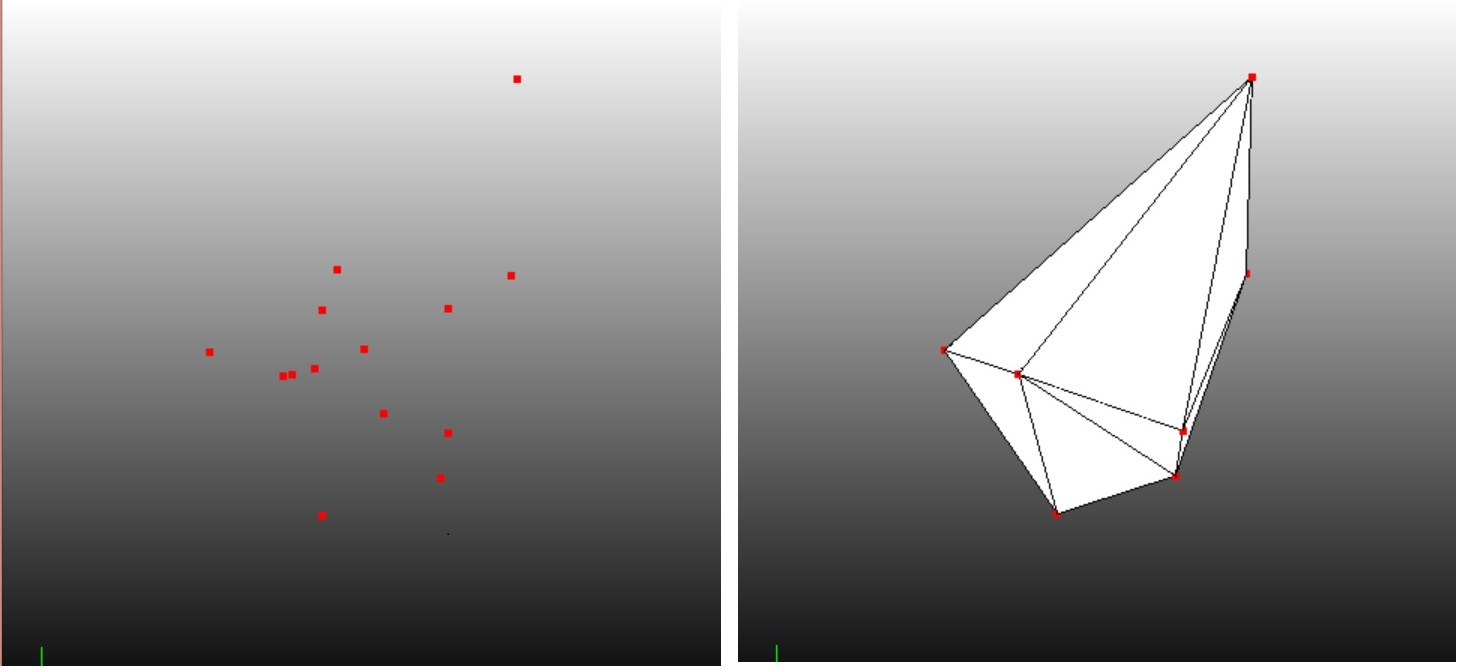
\includegraphics[width=100mm]{point.jpg}\\
  Fig 1. Data point set in 3D and  Deluanay triangulation in 3D(right)
\end{figure}

\begin{figure}[h]
  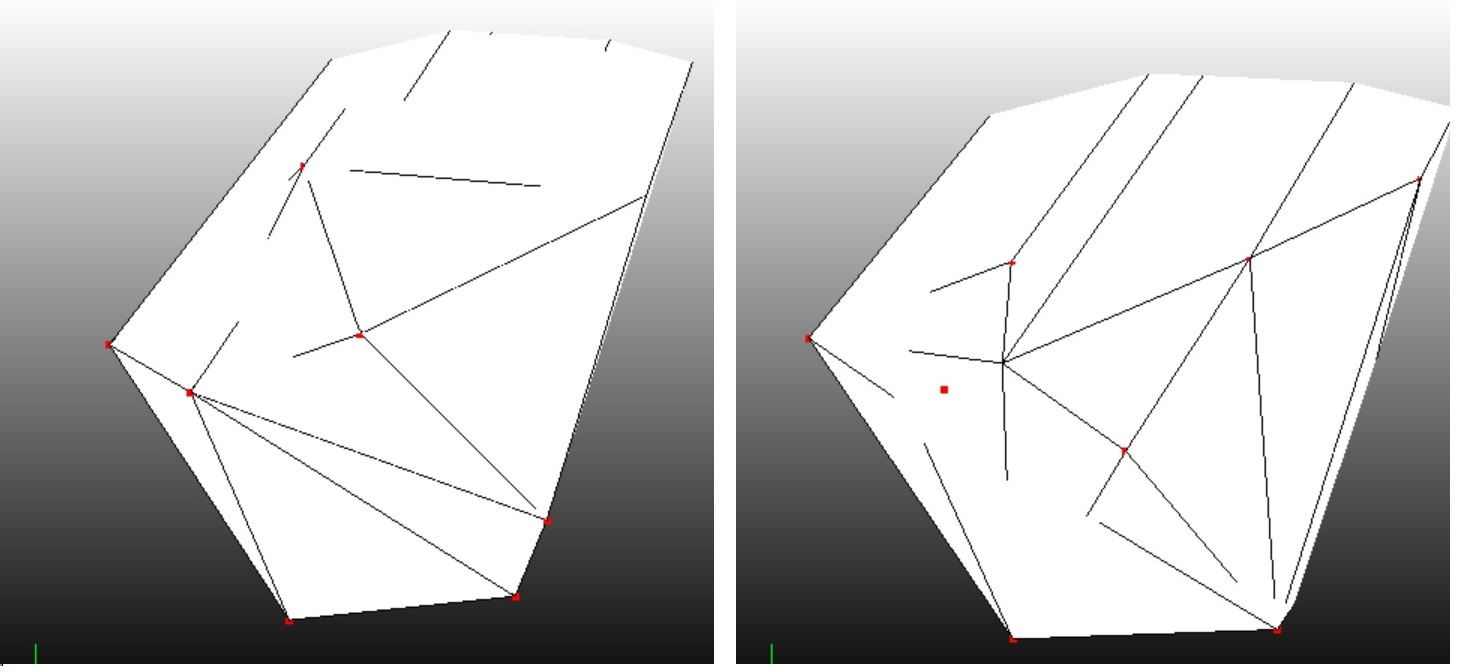
\includegraphics[width=100mm]{tetr.jpg}\\
  Fig 2.Inside picture of tetrahedrons of Deluanay triangulation and Inside picture of facet of Deluanay triangulation(right)
\end{figure}


\section{Known bugs/limitations}
There are bunch of macros here so it was difficult to understand the code easily.
For the edge part which I didn't put the result here. I'll try this. There is also a degenerate case for the cube(in "data" file). The deluanay triangulation of the cube should generate only five tetrahedrons but the output of the triangulation has more than five tetrahedrons.

\begin{figure}[h]
  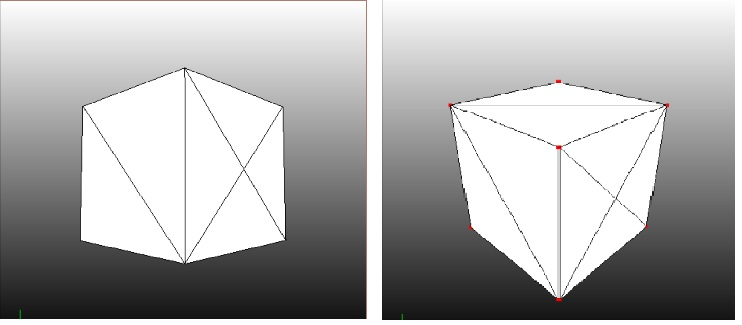
\includegraphics[width=100mm]{degen.jpg}\\
  Fig 3.Degenerate case for the cube.
\end{figure}

\bibliographystyle{plain}
\bibliography{report}

\end{document}


